\documentclass{article}

\RequirePackage{epsfig}

\RequirePackage{graphics}

\ExecuteOptions{dvipsone}

\usepackage{fancyhdr}

\pagestyle{fancy}
\lhead{}
\chead{XBNF Grammars in XMF}
\rhead{\thepage}
\cfoot{(c) 2004 Ceteva Ltd.}

\title{XBNF Grammars in XMF}

\author{Ceteva Ltd.}

\begin{document}

\maketitle

\section{Introduction}

XMF is an environment for constructing advanced software engineering 
tools and applications. A key feature of the XMF environment is the
ability to define {\em domain specific languages} whose features
faithfully represent key aspects of the application domain.

Computer based languages are used as communication media; either system
to system or human to system. In either case, a computer must be able
to recognise phrases expressed in the language. When phrases are presented
to a computer they must be interpreted in some way. Typically, phrases
may be interpreted directly, as they are recognized, or some internal
representation for the phrases may be synthesized (abstract syntax) and
subsequently passed on to an internal module for processing.

There are a variety of formats by which language may be conveyed to a 
computer; a common mechanism is by text. A standard way of defining how
to recognize and process text-based languages is by supplying a {\em grammar}.
A grammar is a collection of rules that define the legal sequences of
text strings in a language. In addition to recognising language phrases,
a grammar may include actions that are to be performed as sub-phrases
are processed.

In order to use grammars to process language phrases we must supply the
grammar to a program called a {\em parser}. The medium used to express the
grammar is usually text. BNF (and te extended version EBNF) is a text-based 
collection of grammar formation rules. BNF defines how to express a grammar
and what the grammar means in terms of processing languages. 

This document describes the XMF version of EBNF, called XBNF. XBNF integrates
EBNF with XOCL (and any language defined by XBNF). XMF provides an XBNF
parser that is supplied with an XBNF grammar and will then parse and synthesize
XMF-defined laguages.

Grammars (and therefore languages) in XMF are associated with classes. Typically 
an XBNF grammar defines how to recognize legal sequences of characters in a 
language and to syntheisize an instance of the associated class (and populate the
instance with instances of the class's attribute types).

\section{Parsing and Synthesizing}

This section describes the basics of using XBNF to define simple grammars
that recognize languages and synthesize XMF data values.

A grammar is an instance of the XMF class {\tt Parser::BNF::Grammar}. A 
grammar consists of a collection of {\em clauses} each of which is a
rule that defines a non-terminal of the grammar. A non-terminal is a
name (by convention a non-terminal name starts with an upper case letter).

A clause has the following form:
\begin{verbatim}
NAME ::= RULE .
\end{verbatim}
where the {\tt RULE} part defines how to recognize a sequence of input
characters. To illustrate the essential elements of a grammar definition
we will build a simple caculator that recognises arithmetic expressions
and executes (synthesizes) the expressions (integers) as the parse proceeds.
The grammar is constructed incrementally and defined as the value of the
global variable {\tt Calculator}:
\begin{verbatim}
Root::Calculator :=
  @Grammar  
\end{verbatim}
Typically, a grammar has a starting non-terminal; this is the clause that
is used as the tsarting point of a parse. There is nothing special about 
the starting non-terminal in the definition. In the case of {\tt Calculator},
the starting non-terminal is {\tt Calc}:
\begin{verbatim}
Calc ::= Mult '='.   
\end{verbatim}
The clause for {\tt Calc} defines that to recognize this non-terminal
a parse must recognize an {\tt Mult} (defined below) followed by a
{\em terminal} {\tt '='}. A terminal is a sequences of characters in 
quotes; a terminal successfully matches an input when the input 
corresponds to exactly the characters, possibly preceded by whitespace.
Therefore, a {\tt Calc} is recognized when a {\tt Mult} is recognized
followed by a {\tt = }.

A {\tt Mult} is a multiplicative expression, possibly involving the 
operators {\tt *} and {\tt /}. We use a standard method of defining
operator precedence in the grammar, where addition operators bind
tighter than multiplicative operators. This is achieved using two different
non-terminals:
\begin{verbatim}
Mult ::= n1 = Add (   
  '*' n2 = Mult { n1 * n2 } |
  '/' n2 = Mult { n1 / n2 } |
  { n1 }      
). 
\end{verbatim}
The clause for {\tt Mult} shows a number of typical grammar features.
A {\tt Mult} is successfully recognized when a {\tt Add} is recognized
followed by an optional {\tt *} or {\tt /} operator.

Each non-terminal synthesizes a value when it successfully recognizes
some input. When one non-terminal {\em calls} another (for example {\tt Add}
is called by {\tt Mult}) the value syntheized by the called non-terminal
may be optionally named in the definition of the calling non-terminal.
Once named, the syntheized value may be referenced in the rest of the 
rule. Naming occurs a number of times in the definition of {\tt Mult}
where the names {\tt n1} and {\tt n2} are used to refer to syntheisized
numbers.

A clause may include optional parts separated by {\tt |}. In general,
if a clause contains an optional component of the form {\tt A | B}
where {\tt A} and {\tt B} are arbitrary components, then a parse
is successful when either {\tt A} or {\tt B} is successful. 

The clause
for {\tt Mult} contains three optional components that occur after the
initial {\tt Add} is successful (hence the need for parentheses around
the optional components to force the {\tt Add} to occur). Once the
{\tt Add} is successful then the parse is successful when one of the 
following occurs:
\begin{itemize}
\item a {\tt *} is encountered followed by a {\tt Mult}.
\item a {\tt +} is encountered followed by a {\tt Mult}.
\item no further input is processed (this option must occur last since
it subsumes the previous two options -- options are tried in turn).
\end{itemize}
Clauses may contain {\em actions}. A action is used to synthesize arbitrary
values and can refer to values that have been named previously in the 
clause. An action is an XOCL expression enclosed in {\tt \{} and {\tt \}}.
Just like calls to non-terminals in the body of a clause, an action
returns a value that may be named. If the last component performed by
the successful execution of a clause is an action then the value produced
by the action is the value returned by the clause.

The clause for {\tt Mult} contains a number of actions that are used
to synthesize values (in this case evaluate numeric expressions).

The clause for {\tt Add} is the same as that for {\tt Mult} except
that the clause recognizes and syntheises addition expressions:
\begin{verbatim}
Add ::= n1 = Int ( 
  '+' n2 = Add { n1 + n2 } |
  '-' n2 = Add { n1 - n2 } |
  { n1 }    
).   
\end{verbatim}
The complete definition of the calculator grammar is given in appendix
\ref{calculator}.

A parse is performed by creating a {\em parsing machine}. A parsing machine
is initialized with the grammar that will control the parse and the input
channel that will supply the characters for the parse. Given a parsing
machine, a parse is performed by running the machine; the name of the
starting non-terminal is supplied for each run. The machine will then run
and terminate in one of two states:
\begin{itemize}
\item the parse is successful and the run returns the value syntheisized by 
the starting non-terminal.
\item the parse is unsuccessful.
\end{itemize}
A parsing machine for the calculator grammar that takes characters from
the standard input is created as follows:
\begin{verbatim}
state := Parser::Machine::State(Calculator,stdin);
\end{verbatim}
Run the machine as follows:
\begin{verbatim}
result := state.run("Calc");
\end{verbatim}
Test whether the parse failed:
\begin{verbatim}
state.failed
\end{verbatim}

\section{Sequences of Elements}

A grammar rule may want to specify that, at a given position in the parse,
a sequence of character strings can occur. For example, this occurs when
parsing XML elements, where a composite element can have any number of
children elements each of which is another element.

XBNF provides the postfix operators {\tt *} and {\tt +} that apply to
a clause component {\tt X} and define that the parse may recognize
sequences of occurrences of {\tt X}. In the case of {\tt *}, there may be
0 or more occurrences of {\tt X} and in the case of {\tt +} there may be
1 or more occurrences of {\tt X}. If {\tt X} synthesizes a value each time it is
used in a parse then the use of {\tt *} and {\tt +} synthesizes sequences
of values, each value in the sequence is a value syntheiszed by {\tt X}.

The following gramar shows an example of the use of {\tt *}. XML elements
are trees; each node in the tree has a label. The following grammar recognizes
XML (without attributes and text elements) trees and synthesizes an XMF
sequence representation for the XML tree. The grammar shows the use of the
builtin non-terminal {\tt Name} that parses XMF names and synthesizes the
name as a string:
\begin{verbatim}
Root::XML :=
  @Grammar
    Element ::= SingleElement | CompositeElement.  
    SingleElement ::= '<' tag = Name '/>' { Seq{tag} }.
    CompositeElement ::= 
      '<' tag = Name '>' 
        children = Element*  
      '<' Name '/>' 
      { Seq{tag | children} }. 
  end; 
\end{verbatim}

\section{Specializing Grammars}

Grammars may be specialized by adding extra clauses or extending existing clauses.
A grammar has an {\tt extends} clause that is followed by comma separated
references to parent grammars. The newly defined grammar is the merge of the
parent grammars and the newly defined clauses. Any clauses in the parents or
in the body of the new definition that have the same names are merged into a single
clause using the {\tt |} operator.

For example, suppose we want to extend the grammar for XML given in the previous
section with the ability to recognize text elements. A text element is supplied
as a string within string-quotes. XBNF provides a built-in non-terminal {\tt Str} for
strings. The new grammar is defined as follows:
\begin{verbatim}
Root::XML2 := 
  @Grammar extends XML 
    Element ::= Str. 
  end;
\end{verbatim}
This is equivalent to the following grammar definition:
\begin{verbatim}
Root::XML :=
  @Grammar
    Element ::= SingleElement | CompositeElement | Str.  
    SingleElement ::= '<' tag = Name '/>' { Seq{tag} }.
    CompositeElement ::= 
      '<' tag = Name '>' 
        children = Element*  
      '<' Name '/>' 
      { Seq{tag | children} }. 
  end; 
\end{verbatim}

\section{Working with Syntax}

Although grammars can be defined to synthesize values of any type, it is
often the case that we want a grammar to synthesize {\em syntax}. This
section describes the XMF execution model and shows how a grammar can be 
used to synthesize abstract syntax.

\begin{figure}
\begin{center}
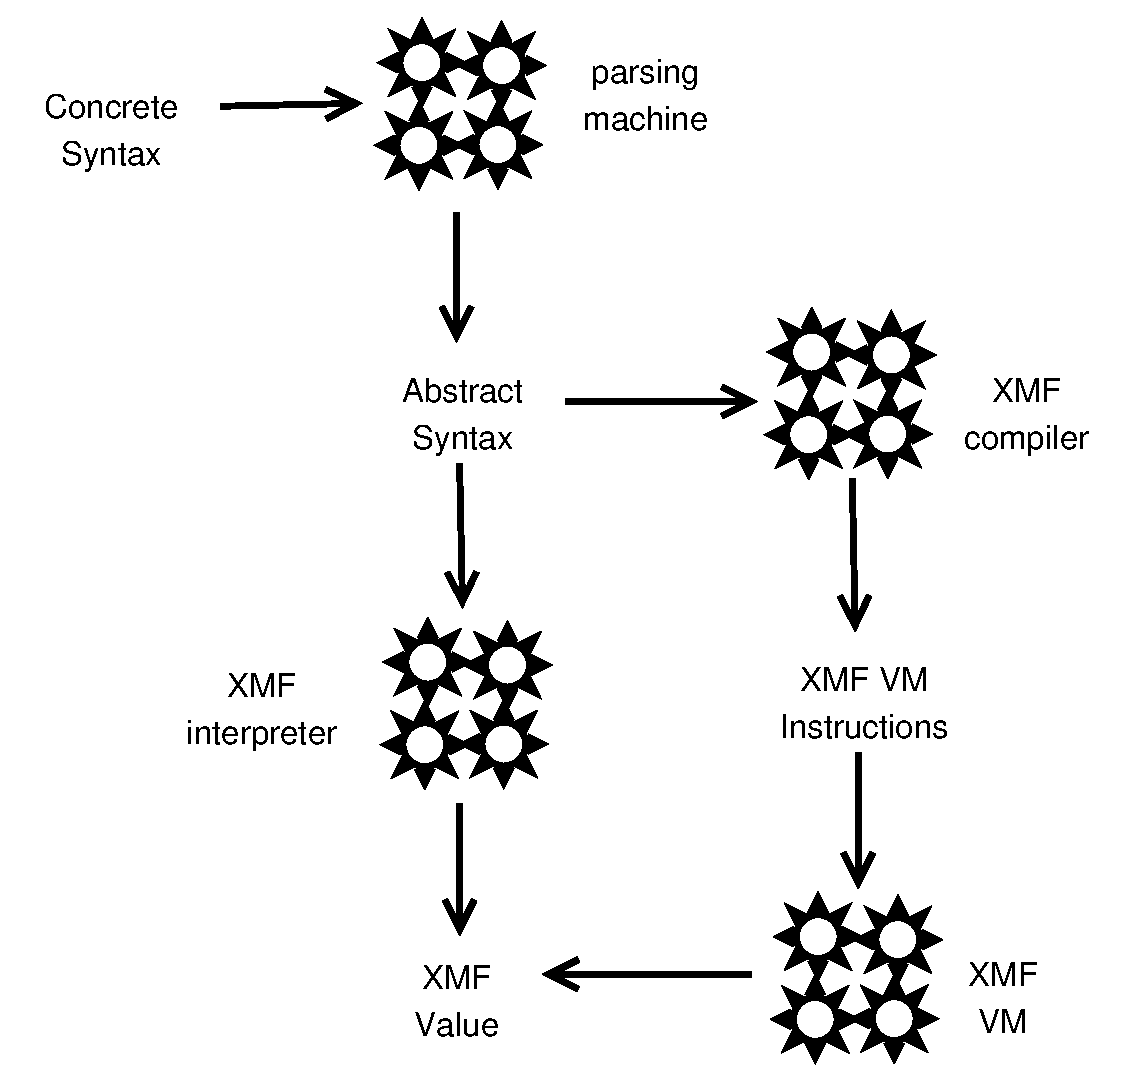
\includegraphics[scale=0.4]{Execution.eps}
\end{center}
\caption{XMF Execution Model}
\label{Execution}
\end{figure}

Consider figure \ref{Execution}. This shows how XMF processes syntax.
Concrete syntax, in the form of character strings in files or typed at
the top-level, are processed by a parsing machine. The parsing machine
determines whether or not the syntax is currently formed and synthesizes
a value. The value produced is abstract syntax.

XMF abstract syntax are objects that are instances of the abstact class
{\tt EMOF::Performable}. The interface defined by {\tt Performable}
requires any concrete sub-class to define operations that support
compilation (to the XMF VM) and evaluation (via the XMF interpreter).

Once abstract syntax has been produced, evaluation may take two routes.
Firstly, syntax may be evaluated directly. In this case the syntax
is supplied to the XMF interpreter together with some context information.
The interpreter recursively processes the abstract syntax tree and produces
an XMF value.

Secondly, syntax may be compiled. the advantage of compiling the syntax is
that compiled code is much more efficient that interpreted code. The
XMF compiler processes the abstract syntax tree and produces a sequence of
XMF VM instructions. At this point the instructions may be written to
a file (the {\tt .o} files produced by the XMF compiler). XMF instructions
are loaded onto the XMF VM and executed to produce an XMF value.

In order to work with this model of execution, XBNF grammars must synthesize
objects of type {\tt Performable}. In many cases a grammar will synthesize
instances of classes defined in the {\tt OCL} package since this is an
extensive programming language. However, an instance of any performable
class (user defined or otherwise) may be produced.

Suppose we want to modify the calculator language defined in appendix
\ref{calculator} to produce the arithmetic expression rather than 
execute the expressions directly. Assuming that the OCL package is imported:
\begin{verbatim}
Root::Calculator :=
  @Grammar
    Calc ::= Mult '='. 
    Mult ::= n1 = Add ( 
      '*' n2 = Mult { BinExp("*",n1,n2) } |
      '/' n2 = Mult { BinExp("/",n1,n2) } |
      { n1 }  
    ). 
    Add ::= i = Int n1 = { IntExp(i) } ( 
      '+' n2 = Add { BinExp("+",n1,n2) } |
      '-' n2 = Add { BinExp("/",n1,n2) } |
      { n1 }  
    ).  
  end;
\end{verbatim}
Alternatively we might choose to use quasi-quotes:
\begin{verbatim}
Root::Calculator :=
  @Grammar
    Calc ::= Mult '='. 
    Mult ::= n1 = Add ( 
      '*' n2 = Mult { [| <n1> * <n2> |] } |
      '/' n2 = Mult { [| <n1> / <n2> |] } |
      { n1 }  
    ). 
    Add ::= i = Int n1 = { IntExp(i) } ( 
      '+' n2 = Add { [| <n1> + <n2> |] } |
      '-' n2 = Add { [| <n1> - <n2> |] } |
      { n1 }  
    ).  
  end;
\end{verbatim}

\section{Language Definition with {\tt @}}

XMF allows grammars to be attached to classes and XBNF allows a grammar {\em G} to permit
the parsing machine that is currently parsing with respect to {\em G} to {\em escape} to
another grammar via the {\tt At} mechanism. Whilst this mechanism is very general,
in most cases it is used with respect to the XOCL grammar {\tt OCL::OCL.grammar}. XOCL
defines that given a grammar for a class {\tt C}, when parsing an XOCL expression, if the
parser encounters an expression of the form:
\begin{verbatim}
@C
  <BODY>
end
\end{verbatim}
then the grammar defined by {\tt C} is used to parse the text {\tt <BODY>}. If the
grammar for {\tt C} is defined as an extension of the XOCL grammar then the {\tt @}
escape also applies while parsing {\tt <BODY>}.

The {\tt @} escape mechanism allows arbitrary languages to be embedded within
XOCL. If used in a lightweight fashion, XOCL can be extended with new language
constructs; for example, this is how {\tt For} and {\tt While} are added to XOCL
in the definition of XMF. If used in a heavyweight fashion, complete languages
can be embedded in XOCL and {\tt @} is used to switch from one language to another;
this has been used to embed MicroJava within XOCL. This section simple examples of 
how to define a lightweight language contruct using the {\tt @} escape mechanism. 

\subsection{A Record Construct}

Consider a requirement for a new record construct
where records have fields; a field consists of a name and a value. Special syntax
is to be provided where the value of a field is an operation. A record is a name-space
for its fields:
\begin{verbatim}
r := 
  @Record
    val x = 100
    op setx(v) me::x := v
  end;
\end{verbatim}
A field of a record is referenced using the standard name-space notation:
\begin{verbatim}
r::x;
\end{verbatim}
produces {\tt 100}. Within operations, a record can reference itself as {\tt me}
(like {\tt self} in XOCL). Operations are just field values; to invoke an
operation reference it and apply it to its argument (limited to a single argument):
\begin{verbatim}
r::setx(1000);
\end{verbatim}
sets the value of the {\tt x} field to {\tt 1000}.

The record language feature is defined as a class called {\tt Record} with an 
appropriate grammar. The grammar synthesizes an XOCL expression that creates
and initialises an instance of the class {\tt Record}. During the parse each
field of the record is synthesized as an instance of the class {\tt Field}:
\begin{verbatim}
context Root
  @Class Field 
    @Attribute name : String end
    @Attribute value : Performable end
    @Constructor(name,value) end
    @Operation nameExp():Performable
      StrExp(name)
    end
    @Operation symbExp():Performable
      [| Symbol(<self.nameExp()>) |]
    end
  end
\end{verbatim}
The class {\tt Field} has two attributes: {\tt name} is the name of the field
and {\tt value} is an expression. The value expression denotes an operation
of one argument that is supplied with an instance of the class {\tt Record}
and returns the value of the field. Names of fields in records are symbols
(actually a record will be a name-space: typically names in name-spaces
are symbols in order to make name lookup efficient), since the parser recognizes
a field name as a string, this is turned into a symbol {\em expression} using
the operation {\tt symbExp}.

The class {\tt Record} defines a grammar that parses record expressions. Instances
of the class {\tt Record} are name-spaces that associate field names (symbols)
with field values. A record (unlike record expressions) does not make a distinction
between value fields and operation fields. The class has comments in-line:
\begin{verbatim}
context Root
  @Class Record extends NameSpace
  
    // The grammar extends the XOCL grammar in order to allow
    // references to the non-terminal Exp for field values...
    
    @Grammar extends OCL::OCL.grammar
      Record ::= fields = Field* {
      
        // Synthesize an expression that creates and 
        // initialises a record. Records a name-spaces
        // so we can add names and their values using
        // the 'add/2' operation. The names are symbols
        // and the values of fields are always operations
        // that are supplied with the record as the value
        // of 'me' (used only by operation fields)...
        
        [| let record = Record()
           in <fields->iterate(f r = [| record |] |
                [| <r>.add(<f.symbExp()>,<f.value>(record)) |])>
           end
        |]
      }.
      Field ::= ValueField | OpField.
      
      // All field values expect to be supplied with a 
      // record for the value of 'me'. A value field
      // will just ignore the value of me...
      
      ValueField ::= 'val' name = Name '=' value = Exp { 
        Field(name,[| @Operation(me) <value> end |]) 
      }.
      
      // An operation field is supplied with the value of
      // 'me' and returns an operation. Since arguments are
      // lexically scoped, 'me' is available in the body of
      // the field operation...
      
      OpField ::= 'op' name = Name '(' arg = Name ')' '=' body = Exp { 
        Field(name,[| @Operation(me) @Operation(<arg>) <body> end end |]) 
      }.
    end
  end
\end{verbatim}

\subsection{A For Loop}

New language constructs are often defined as translations to existing language constructs.
This is sometimes referred to as {\em syntactic sugar} and the process of translation
from new abstract syntax construct to old abstract syntax construct is referred to
as {\em desugaring}. This section shows a simple example of sugar by defining a {\tt For}
loop that translates to a {\tt While} loop.

A {\tt For} loop is to have a controlled variable ({\tt name}), a collection ({\tt coll}) and
a body ({\tt body}). The loop selects elements from the collection in turn, binds them to
the controlled variable and performs the body:
\begin{verbatim}
context Root
  @Class For extends Sugar
    @Attribute name : String end
    @Attribute coll : Performable end
    @Attribute body : Performable end 
    @Constructor(name,coll,body) end
  end
\end{verbatim}
The grammar for the new language construct creates a new instance of the class {\tt For}:
\begin{verbatim}
context For
  @Grammar extends OCL::OCL.grammar
    For ::= name = Name 'in' coll = Exp 'do' body = Exp { 
      For(name,coll,body) 
    }.
  end
\end{verbatim}  
Classes that inherit from {\tt XOCL::Sugar} must define an operation named {\tt desugar}.
This is called by all clients of the {\tt Performable} interface when the new language
construct is to be evaluated or compiled. The operation {\tt desugar} returns an
instance of the class {\tt Performable}:
\begin{verbatim}
@Operation desugar()
  [| let forColl = <coll>;
         isFirst = true
     in @While not forColl->isEmpty do
          let <name> = forColl->sel
          in forColl := forColl->excluding(<Var(name)>);
             let isLast = forColl->isEmpty
             in <body>;
                isFirst := false
             end
          end
        end
     end
  |]
end
\end{verbatim}

\subsection{A Block Feature}

XOCL does not provide a {\em goto} language feature. Although goto is not usually
considered good programming practice; it can be convenient when implementing certain
well-understood tasks that need to be efficient (flow control can always be achieved
using first class operations, however there is a price to pay in terms of speed and
space).

Consider a new language feature for blocks. A block contains a sequence of XOCL
expressions (referred to as {\em statements}). Each statement may be optionally 
labelled. A block may contain one or more guarded jumps. A guarded jump consists 
of a predicate expression and a label. Execution of a block proceeds by executing 
each statement in turn. On encountering a guarded jump, if the predicate expression is
true then execution jumps to the appropriate labelled statement. For example:
\begin{verbatim}
context Root
  @Operation countDown(x)  
    @Block
      [decx] x := x - 1;
      x.println();
      ? x > 10 go decx;
    end
  end
\end{verbatim}
Since XOCL does not provide a goto feature, we must implement blocks by extending the
XOCL compiler. Fortunately, this is not as drastic as it sounds. We need to know a
small amount about the compiler interface and a few XMF VM instructions. The compiler
will produce the following code for {\tt countDown}:
\begin{verbatim}
Label     Instr              Comment
-------------------------------------
                             // Entry code for the operation ...
DECX      NOOP               // Label
                             // Code to decrement x
                             // Code to print x
                             // Code to test x > 10
          NEGATE
          SKIPFALSE JMPDECX  // Jump indirectly to DECX
          SKIP END           // Leave the operation
                             // Start of label table...
JMPDECX   SKIPBACK DECX      // Jump directly to DECX
END       NOOP
\end{verbatim}
It is worth noting in the schematic for XMF VM instructions above that:
\begin{itemize}
\item all VM instructions can be labelled with a string.
\item conditional skip instructions can only go {\em forward} hence the use of a label table
at the end of the block.
\item {\tt NOOP} instructions are used as placeholders for labels (they are ignored by the 
XMF VM).
\end{itemize}
The {\tt Block} feature is implemented using a grammar that extends the XOCL grammar.
There are three types of component in a block: a {\em raw} expression; a {\em labelled}
expression and a {\em jump}. Each component is to be compiled and therefore must implement
the {\tt Performable} interface: {\tt FV}, {\tt maxLocals} and {\tt compile}. 
Furtunately, we don't need to know much about these operations since block components
are just wrappers for XOCL expressions:   
\begin{verbatim}
context Root
  @Class RawExp extends Performable
    @Attribute exp : Performable end
    @Constructor(exp) end
    @Operation FV()
      exp.FV()
    end
    @Operation maxLocals():Integer
      exp.maxLocals()
    end
    @Operation compile(e,f,l,s):Seq(Instr)
      exp.compile(e,f,l,s)
    end
  end
\end{verbatim}
A labelled expression is the same as a raw expression except that it adds a dummy {\tt NOOP}
instruction with the supplied label:
\begin{verbatim}
context Root
  @Class LabelledExp extends RawExp
    @Attribute label : String end
    @Constructor(label,exp) end
    @Operation compile(e,f,l,s):Seq(Instr)
      Seq{NoOp().setLabel(label)} + super(e,f,l,s)
    end
  end
\end{verbatim}
A jump statement jumps to the appropriate element in the label table. Jumps in
blocks are performed indirectly because the label may occur before or after the
jump statement, but XMF conditional skip instructions can only move forward
in the instruction stream (actually not true, but the alternative is to calculate
offsets by counting instructions).
\begin{verbatim}
context Root
  @Class Jump
    @Attribute guard : Performable end
    @Attribute label : String end
    @Constructor(guard,label) end
    @Operation FV()
      guard.FV()
    end
    @Operation maxLocals():Integer
      guard.maxLocals()
    end
    @Operation compile(e,f,l,s):Seq(Instr)
      guard.compile(e,f,l,s) + 
      Seq{Negate(),SkipFalse("JMP" + label)}
    end
  end
\end{verbatim}
A block is a sequence of statements. A statement may be a raw expression,
a labelled expression or a jump. Each statement is followed by a {\tt ;}
(block expressions are therefore defined by the OCL non-terminal {\tt LogicalExp}
which does not allow {\tt ;} as an expression sequencing operation):
\begin{verbatim}
context Block
  @Grammar extends OCL::OCL.grammar
    Block ::= statements = (RawExp | LabelledExp | Jump)* { 
      Block(statements) 
    }.
    RawExp ::= e = LogicalExp ';' { 
      RawExp(e) 
    }.
    LabelledExp ::= '[' label = Name ']' e = LogicalExp ';' { 
      LabelledExp(label,e) 
    }.
    Jump ::= '?' guard = LogicalExp 'go' label = Name ';' { 
      Jump(guard,label) 
    }.
  end
\end{verbatim}
The class {\tt Block} is a sub-class of {\tt Performable} and therefore
implements the operations {\tt FV}, {\tt maxLocals} and {\tt compile}.
To compile a block we compile the individual statements; each statement
produces a sequence of instructions which are concatenated together using
{\tt flatten}. Instructions for the jump table are added to the end of the
block instructions:
\begin{verbatim}
context Root
  @Class Block extends Performable
    @Attribute statements : Seq(Element) end
    @Constructor(statements) ! end
    @Operation FV():Set(String)
      statements->asSet->collect(s | s.FV())->flatten
    end
    @Operation maxLocals()
      statements->collect(s | s.maxLocals())->max
    end
    @Operation compile(e,f,l,s):Seq(Instr)
      statements->collect(s | s.compile(e,f,false,s))->flatten +
      Seq{Skip("END")} +
      self.jmpTable() +
      Seq{NoOp().setLabel("END")}
    end
    @Operation jmpTable():Seq(Instr)
      statements
        ->select(s | s.isKindOf(LabelledExp))
        ->collect(l | SkipBack(l.label).setLabel("JMP" + l.label)) 
    end
  end
\end{verbatim}
The actual code produced by the compiler for {\tt countDown} is:
\begin{verbatim}
[0000] NOOP
[0001] SOURCEPOS    146  19
[0002] LOCALREF     0
[0003] PUSHINT      1
[0004] SUB
[0005] SETLOCAL     0
[0006] STARTCALL
[0007] SENDLOCAL    0    println 0
[0008] SOURCEPOS    148  9
[0009] LOCALREF     0
[0010] PUSHINT      10
[0011] GREATER
[0012] NEGATE
[0013] SKIPFALSE    1
[0014] SKIP         1
[0015] SKIPBACK     15
[0016] NOOP
[0017] RETURN
\end{verbatim}

\section{Conclusion}

This note has described the key features of XBNF by giving examples of new language
features defined as XBNF grammars. The XBNF grammar for XBNF is defined in appendix
\ref{XBNFGrammar}.

\appendix

\section{A Calculator}

\label{calculator}

\begin{verbatim}
Root::Calculator :=
  
  @Grammar
    
    Calc ::= Mult '='.
      
    Mult ::= n1 = Add (
      
       '*' n2 = Mult { n1 * n2 } |
      '/' n2 = Mult { n1 / n2 } |
      { n1 }
        
    ).
      
    Add ::= n1 = Int (
      
      '+' n2 = Add { n1 + n2 } |
      '-' n2 = Add { n1 - n2 } |
      { n1 }
        
    ).
      
  end;
\end{verbatim}

\section{XBNF Grammar}

\label{XBNFGrammar}

\begin{verbatim}

Action ::= 
  '{' exp = Exp '}' 
  { PreAction(exp) } |
  '?' boolExp = Exp
  { PrePredicate(boolExp) }.
    
Atom ::= 
  Action    | 
  Literal   | 
  Call      | 
  Not       | 
  '(' Disjunction ')'.
  
Binding ::= 
  name = Name '=' atom = Sequence { 
    And(atom,Bind(name)) 
  }.
    
Call ::= 
  name = Name { Call(name) }.
  
Clause ::= 
  name = Name '::=' body = Disjunction '.' { Clause(name,body) }. 
  
Conjunction ::= 
  elements = Element+ { 
    elements->tail->iterate(e conj = elements->head | 
      And(conj,e)) 
  }. 
  
Disjunction ::= 
  element = Conjunction [ 
    '|' rest = Disjunction element = { Or(element,rest) } 
  ] 
  { element }.
   
Element ::= 
  Optional  | 
  Binding   | 
  Sequence.
  
Grammar ::= 
  parents = GrammarParents
  imports = GrammarImports
  clauses = Clause* { Grammar(parents,clauses->asSet,"",imports) }.
  
GrammarImports ::= 
  'import' class = Exp classes = (',' Exp)* { Seq{class | classes} } |
  { Seq{} }.
  
GrammarParents ::= 
  'extends' parent = Exp parents = (',' Exp)* { 
     parents->asSet->including(parent) 
   } |
  { Set{} }.

Literal ::= 
  'Char'       { Char() }     |
  'Str'        { Str() }      | 
  'Terminal'   { Term() }     |
  'Token'      { Tok() }      |
  'Int'        { Int() }      | 
  'Name'       { Name() }     | 
  'EOF'        { EOF() }      | 
  '@'          { At() }       |
  'ImportAt'   { ImportAt() } |
  terminal = Terminal { Terminal(terminal) }.
       
Not ::= 'Not' '(' parser = Sequence ')' { Not(parser) }.

Optional ::= 
  '[' opt = Disjunction ']'
  { Opt(opt) }.
  
Path ::= name = Name names = ('::' Name)* { Seq{name | names} }.
    
TypeCheck ::=
  element = Atom [ 
    ':' type = Path element = { And(element,TypeCheck(type)) } 
  ] { element }.
  
Sequence ::= 
  element = TypeCheck [ 
    '*' element = { StarCons(element) } | 
    '+' element = { PlusCons(element) } ] 
  { element }.
\end{verbatim}

\end{document}